\documentclass[11pt, a4paper]{ctexart}
\usepackage{amsmath, amssymb, amsthm}
\usepackage{geometry}
\usepackage{graphicx}
\usepackage{xcolor}
\usepackage{hyperref}
\usepackage{listings}
\usepackage{hyperref}
% 页面布局
\geometry{a4paper, left=2.5cm, right=2.5cm, top=2.5cm, bottom=2.5cm}

\hypersetup{
hidelinks,
colorlinks=true,
allcolors=black,
pdfstartview=Fit,
breaklinks=true
}

% 中文定理环境
\theoremstyle{definition}
\newtheorem{definition}{定义}[section]
\newtheorem{example}{例}[section]
\newtheorem{exercise}{练习}[section]

\theoremstyle{plain}
\newtheorem{theorem}{定理}[section]
\newtheorem{lemma}[theorem]{引理}
\newtheorem{proposition}[theorem]{命题}
\newtheorem{corollary}{推论}

\definecolor{mygreen}{rgb}{0,0.6,0}
\definecolor{mygray}{rgb}{0.5,0.5,0.5}
\definecolor{mymauve}{rgb}{0.58,0,0.82}

\lstset{ %
  backgroundcolor=\color{white},   % choose the background color; you must add \usepackage{color} or \usepackage{xcolor}
  basicstyle=\footnotesize,        % the size of the fonts that are used for the code
  breakatwhitespace=false,         % sets if automatic breaks should only happen at whitespace
  breaklines=true,                 % sets automatic line breaking
  captionpos=bl,                    % sets the caption-position to bottom
  commentstyle=\color{mygreen},    % comment style
  deletekeywords={...},            % if you want to delete keywords from the given language
  escapeinside={\%*}{*)},          % if you want to add LaTeX within your code
  extendedchars=true,              % lets you use non-ASCII characters; for 8-bits encodings only, does not work with UTF-8
  frame=single,                    % adds a frame around the code
  keepspaces=true,                 % keeps spaces in text, useful for keeping indentation of code (possibly needs columns=flexible)
  keywordstyle=\color{blue},       % keyword style
  language=c++,                 % the language of the code
  morekeywords={*,...},            % if you want to add more keywords to the set
  numbers=left,                    % where to put the line-numbers; possible values are (none, left, right)
  numbersep=5pt,                   % how far the line-numbers are from the code
  numberstyle=\tiny\color{mygray}, % the style that is used for the line-numbers
  rulecolor=\color{black},         % if not set, the frame-color may be changed on line-breaks within not-black text (e.g. comments (green here))
  showspaces=false,                % show spaces everywhere adding particular underscores; it overrides 'showstringspaces'
  showstringspaces=false,          % underline spaces within strings only
  showtabs=false,                  % show tabs within strings adding particular underscores
  stepnumber=1,                    % the step between two line-numbers. If it's 1, each line will be numbered
  stringstyle=\color{orange},     % string literal style
  tabsize=2,                       % sets default tabsize to 2 spaces
  %title=myPython.py                   % show the filename of files included with \lstinputlisting; also try caption instead of title
}

% 自定义命令
\newcommand{\R}{\mathbb{R}}
\newcommand{\C}{\mathbb{C}}
\newcommand{\diff}{\mathop{}\!\mathrm{d}}

\title{Kokkos Trilinos 学习}
\author{曾祥磊}
\date{\today}

\begin{document}
\maketitle
\tableofcontents

\newpage
\section{Kokkos 学习}
\subsection{Kokkos Tutorial}

为了打代码和公式方便,使用\LaTeX 进行排版。书接上文,
在完成了Kokkos的安装和使用后,我们已经能够正常的使用
Kokkos进行并行计算。从教程开始学习Kokkos的使用方法,
gemm算法,SIMD指令,CrsMatrix,SparseMatrix,CG,GMRES
,欧拉流的FVM求解。

Kokkos目前用的人不多,但在开源HPC套件里面逐步适配,目前我
了解和使用过的是Trilinos(sandia老本家),分子动力学软件LAMMPS
(想不到吧,这也是sandia本家的),Petsc套件的GPU支持。这帮人里面
有不少c++委员会的人,拉起了一个提案,为在c23标准下为c++的STL提供一个
多维数组的接口,实现矩阵向量和张量计算,包含在std::mdspan中。

如果你这两个都用过,会非常惊奇的发现(这俩一帮人写的)用法和模板参数几乎
一致。如下为mdspan和kokkos的核心模板参数,基本上包括参数类型,多维数组的长度,
排布方式,访问方式。

\begin{lstlisting}
  template <class T,
            class Extents,
            class LayoutPolicy = std::layout_right, 
            class AccessorPolicy = std::default_accessor<T>> 
\end{lstlisting}

\begin{lstlisting}
template <class DataType 
       [, class LayoutType] 
       [, class MemorySpace] 
       [, class MemoryTraits]>
  class View
  {
    ...
  };
\end{lstlisting}

既然都搞定矩阵表示了,为什么不把矩阵向量计算顺带也搞定。巧了,这帮人也是这么
想的,除了mdspan提案,还将在c26标准中,实现blas的所有功能,包含在std::linalg
头文件中,作为mdspan的延申。

\subsubsection{Tutorial Step 1}
Kokkos的练习代码包括两个部分,第一部分为原始的没有改为并行的
代码,第二部分为改为并行后的修正代码,在此将原始代码保存为注释
,修改后代码为正常运行代码。
\begin{lstlisting}
#include <limits>
#include <cmath>
#include <cstdio>
#include <cstdlib>
#include <cstring>
#include <iostream>
#include <Kokkos_Core.hpp>

// 检查命令行输入的N,M,S是否符合要求,nrepeat表示其重复计算次数
void checkSizes(int &N, int &M, int &S, int &nrepeat);

int main(int argc, char *argv[])
{
    int N = -1;
    int M = -1;
    int S = -1;
    int nrepeat = 100;

    // 命令行参数读取
    for (int i = 0; i < argc; i++)
    {
    if ((strcmp(argv[i], "-N") == 0) || (strcmp(argv[i], "-Rows") == 0))
    {
        N = pow(2, atoi(argv[++i]));
        std::cout << "  User N is " << N << std::endl;
    }
    else if ((strcmp(argv[i], "-M") == 0) || (strcmp(argv[i], "-Columns") == 0))
    {
        M = pow(2, atof(argv[++i]));
        std::cout << "  User M is " << M << std::endl;
    }
    else if ((strcmp(argv[i], "-S") == 0) || (strcmp(argv[i], "-Size") == 0))
    {
        S = pow(2, atof(argv[++i]));
        std::cout << "  User S is " << S << std::endl;
    }
    else if (strcmp(argv[i], "-nrepeat") == 0)
    {
        nrepeat = atoi(argv[++i]);
    }
    else if ((strcmp(argv[i], "-h") == 0) || (strcmp(argv[i], "-help") == 0))
    {
        std::cout << "y^T*A*x Options: " << std::endl;
        std::cout << "-Rows (-N) <int>:      rows (default: 4096) " << std::endl;
        std::cout << "-Columns (-M) <int>:   columns (default: 1024) " << std::endl;
        std::cout << "-Size (-S) <int>:      matrix (default: N*M ) " << std::endl;
        std::cout << "-nrepeat <int>:        repeats (default: 100) "<< std::endl;
        std::cout << "-help (-h):            print this message " << std::endl;
        exit(1);
    }
    }

    // 检查参数是否合规
    checkSizes(N, M, S, nrepeat);

    // Kokkos环境初始化,和MPI_Initialize用法一致,所以代码都需要在
    // Initialize和Finalize之间
    Kokkos::initialize(argc, argv);
    {
    // 检测可用并行空间
    // EXERCISE give-away: Choose an Execution Space.
    // using ExecSpace = Kokkos::Serial;
    // using ExecSpace = Kokkos::Threads;
    // using ExecSpace = Kokkos::OpenMP;
    // using ExecSpace = Kokkos::Cuda;

    // EXERCISE: Choose device memory space.
    // using MemSpace = Kokkos::HostSpace;
    // using MemSpace = Kokkos::CudaSpace;
    // using MemSpace = Kokkos::CudaUVMSpace;

    #ifdef KOKKOS_ENABLE_CUDA
    #define MemSpace Kokkos::CudaSpace
    #endif

    #ifdef KOKKOS_ENABLE_HIP
    #define MemSpace Kokkos::Experimental::HIPSpace
    #endif

    #ifdef KOKKOS_ENABLE_OPENMPTARGET
    #define MemSpace Kokkos::OpenMPTargetSpace
    #endif

    #ifndef MemSpace
    #define MemSpace Kokkos::HostSpace
    #endif

    // 并行空间
    using ExecSpace = MemSpace::execution_space;
    
    // EXERCISE give-away: Use a RangePolicy.
    // using range_policy = Kokkos::RangePolicy<ExecSpace>;
    // 执行策略,在此模板只指定了并行空间
    using range_policy = Kokkos::RangePolicy<ExecSpace>;

    // EXERCISE give-away: Choose a Layout.
    // EXERCISE: When exercise is correctly implemented, then
    //           either layout will generate the correct answer.
    //           However, performance will be different!

    // using Layout = Kokkos::LayoutLeft;
    using Layout = Kokkos::LayoutRight;

    // Allocate y, x vectors and Matrix A on device.
    // EXERCISE: Use MemSpace and Layout.
    // Kokkos::View是Kokkos的通用的数组类型,类似std::shared_ptr
    // 1D可以视为向量类型,2D视为矩阵类型
    using ViewVectorType = Kokkos::View<double *, Layout, MemSpace>;
    using ViewMatrixType = Kokkos::View<double **, Layout, MemSpace>;

    // 定义需要的矩阵A和向量y,x
    // 传入的字符串作为lable唯一的确定对应的实例,在debug中非常有效
    ViewVectorType y("y", N);
    ViewVectorType x("x", M);
    ViewMatrixType A("A", N, M);

    // CUDA中的数据不能被CPU访问和读取,如果需要进行改动,需要先创建
    // CPU可访问的数据,也就是ViewVectorType::HostMirror
    ViewVectorType::HostMirror h_y = Kokkos::create_mirror_view(y);
    ViewVectorType::HostMirror h_x = Kokkos::create_mirror_view(x);
    ViewMatrixType::HostMirror h_A = Kokkos::create_mirror_view(A);
    
    // 初始化y 
    for (int i = 0; i < N; ++i)
    {
        h_y(i) = 1;
    }

    // 初始化x 
    for (int i = 0; i < M; ++i)
    {
        h_x(i) = 1;
    }

    // 初始化A 
    for (int j = 0; j < N; ++j)
    {
        for (int i = 0; i < M; ++i)
        {
        h_A(j, i) = 1;
        }
    }

    // 由CPU可访问空间转移到对应的并行空间
    Kokkos::deep_copy(y, h_y);
    Kokkos::deep_copy(x, h_x);
    Kokkos::deep_copy(A, h_A);

    // 计时器
    Kokkos::Timer timer;

    for (int repeat = 0; repeat < nrepeat; repeat++)
    {

        double result = 0;

        // 将yAx分解为y(j) * \sum_{i=0,M} A(j,i) * x(i)
        // range_policy(start,end,...)指定起始和结束index
        // KOKKOS_LAMBDA自动根据并行空间指定LAMBDA函数的初始化类型
        Kokkos::parallel_reduce("yAx", range_policy(0, N), 
        KOKKOS_LAMBDA (int j, double &update) {
        double temp2 = 0;

        for ( int i = 0; i < M; ++i ) {
        temp2 += A( j, i ) * x( i );
        }

        update += y( j ) * temp2; }, result);

        if (repeat == (nrepeat - 1))
        {
        std::cout << "  Computed result for " << N 
                    << " x " << M << " is " << result << std::endl;
        }
    }
    // 计算时间
    double time = timer.seconds();
    // 计算带宽
    double Gbytes = 1.0e-9 * double(sizeof(double) * (M + M * N + N));

    std::cout << "  N( " << N << " ) "
              << "  M( " << M << " ) "
              << "  nrepeat ( " << nrepeat << " ) "
              << "  problem( " << Gbytes * 1000 << " MB ) "
              << "  time( " << time << " s ) "
              << "  bandwidth( " << Gbytes * nrepeat / time << " GB/s )" << std::endl;
    }
    // 结束Kokkos
    Kokkos::finalize();

    return 0;
}

void checkSizes(int &N, int &M, int &S, int &nrepeat)
{

    if (S == -1 && (N == -1 || M == -1))
    {
    S = pow(2, 22);
    if (S < N)
        S = N;
    if (S < M)
        S = M;
    }

    if (S == -1)
    S = N * M;

    if (N == -1 && M == -1)
    {
    if (S > 1024)
    {
        M = 1024;
    }
    else
    {
        M = S;
    }
    }

    if (M == -1)
    M = S / N;

    if (N == -1)
    N = S / M;
}
\end{lstlisting}

\subsubsection{Tutorial Step 2}
这个教程主要介绍不同的储存顺序对于计算性能的影响,尤其是对于不同的架构
而言,对于CPU来说,由于其有缓存机制,每次读取都不会单独读取一个,而是
一次性读取相邻内存上的多个值放入缓存,那么在计算矩阵向量乘法的时候,
在遍历矩阵的列时,每次读取多个列值进行计算,整行计算完成后,步进到下一
行。对于GPU来说,由于存在合并访问机制,理想情况下合并效为100,
否则会浪费大部分的带宽,所以为列优先(GPU部分比较胡编乱造,只能说看个乐)。
\begin{lstlisting}
#include <Kokkos_Core.hpp>
#include <Kokkos_Timer.hpp>
#include <iostream>
#include <cstdio>
// 并行空间
using MemSpace = Kokkos::CudaSpace;

// 二维的数组类型,LayoutLeft -> 列优先,LayoutRight -> 行优先
// 对于CPU来说,矩阵Axb的过程中会大量读取和b中的值,为了提高
// 计算效率,如果Axb中读取一次就可以得到A(i,j)->A(i,j+n)无疑
// 会大大提高计算效率(Cache),对应的是行优先。进一步,如果一次将这读取的
// n个数一起计算,会有极为可观的收益(SIMD) 
// 对GPU来说,GPU核心非常多,由于存在合并访问,行优先会浪费很多的带宽,
// 一般是列优先
using left_type = Kokkos::View<double **, Kokkos::LayoutLeft, MemSpace>;
using right_type = Kokkos::View<double **, Kokkos::LayoutRight, MemSpace>;

using view_type = Kokkos::View<double *, MemSpace>;

// a.extent(0),a.extent(1)指的是View的维数大小,NxM的N和M
template <class ViewType>
struct init_view
{
    ViewType a;
    init_view(ViewType a_) : a(a_) {}

    using size_type = typename ViewType::size_type;

    KOKKOS_INLINE_FUNCTION
    void operator()(const typename ViewType::size_type i) const
    {
    for (size_type j = 0; j < static_cast<size_type>(a.extent(1)); ++j)
    {
        a(i, j) = 1.0 * a.extent(0) * i + 1.0 * j;
    }
    }
};

template <class ViewType1, class ViewType2>
struct contraction
{
    view_type a;
    typename ViewType1::const_type v1;
    typename ViewType2::const_type v2;
    contraction(view_type a_, ViewType1 v1_, ViewType2 v2_)
        : a(a_), v1(v1_), v2(v2_) {}

    using size_type = typename view_type::size_type;

    KOKKOS_INLINE_FUNCTION
    void operator()(const view_type::size_type i) const
    {
    for (size_type j = 0; j < static_cast<size_type>(a.extent(1)); ++j)
    {
        a(i) = v1(i, j) * v2(j, i);
    }
    }
};

// 向量内积
struct dot
{
    view_type a;
    dot(view_type a_) : a(a_) {}
    using value_type = double;
    KOKKOS_INLINE_FUNCTION
    void operator()(const view_type::size_type i, double &lsum) const
    {
    lsum += a(i) * a(i);
    }
};

int main(int argc, char *argv[])
{
    Kokkos::initialize(argc, argv);
    {
    int size = 10000;
    view_type a("A", size);

    // Define two views with LayoutLeft and LayoutRight.
    left_type l("L", size, 10000);
    right_type r("R", size, 10000);

    // Initialize the data in the views.
    Kokkos::parallel_for(size, init_view<left_type>(l));
    Kokkos::parallel_for(size, init_view<right_type>(r));
    // MPI_Barrier
    Kokkos::fence();

    Kokkos::Timer time1;
    Kokkos::parallel_for(size, contraction<left_type, right_type>(a, l, r));
    Kokkos::fence();
    double sec1 = time1.seconds();

    double sum1 = 0;
    Kokkos::parallel_reduce(size, dot(a), sum1);
    Kokkos::fence();

    Kokkos::Timer time2;
    Kokkos::parallel_for(size, contraction<right_type, left_type>(a, r, l));
    Kokkos::fence();
    double sec2 = time2.seconds();

    double sum2 = 0;
    Kokkos::parallel_reduce(size, dot(a), sum2);

    printf("Result Left/Right %f Right/Left %f (equal result: %i)\n", sec1,
            sec2, sum2 == sum1);    
    }
    Kokkos::finalize();
}
\end{lstlisting}

\subsubsection{Tutorial Step 3 - GEMM and Euler Flow}
这个案例主要是使用GEMM算法快速计算矩阵和矩阵的乘法,主要看不懂的点集中在模板化,和一堆
这个作者自己定义的类型上面,之前用Trilinos的时候也是差不多这样坐牢,纯纯的坐牢,想不做
是不可能的,感觉不如Petsc使用起来上手。其次就是CRS矩阵的具体实现过程,如果有兴趣可以参考
注释看一下,sandia实验室的代码都一个样子,封装完成后使用List进行具体实现。

虽然到现在我还是对Kokkos这东西一脸懵逼,但还是要挖个大坑,计划搞明白
这个使用Kokkos,FVM和DG计算时变欧拉流的代码,目前已经能够完全跑起来,使用paraview进行
后处理,可能得补以下FVM的东西,DG之前就看过。在这个过程中连带这学一下Kokkos的稀疏矩阵和
一些抽象的simd指令。

\begin{lstlisting}
#include <limits>
#include <cstdio>
#include <cstdlib>
#include <cstring>

#include <Kokkos_Core.hpp>
#include <KokkosSparse_CrsMatrix.hpp>
#include <KokkosSparse_spgemm.hpp>

void checkSizes(int &N)
{
    // If N is undefined, set it to 2^10 = 1024.
    if (N == -1)
    N = 1024;

    printf("  Number of Rows N = %d, Number of Cols N = %d, Total nnz = %d\n", N, N, 2 + 3 * (N - 2) + 2);

    // Check sizes.
    if (N < 0)
    {
    printf("  Sizes must be greater than 0.\n");
    exit(1);
    }
}

// 这模板外一堆加上参数传入过程,一眼丁真,遮沙避风了
template <typename crsMat_t>
void makeSparseMatrix(
    typename crsMat_t::StaticCrsGraphType::row_map_type::non_const_type &ptr,
    typename crsMat_t::StaticCrsGraphType::entries_type::non_const_type &ind,
    typename crsMat_t::values_type::non_const_type &val,
    typename crsMat_t::ordinal_type &numRows,
    typename crsMat_t::ordinal_type &numCols,
    typename crsMat_t::size_type &nnz,
    const int whichMatrix)
{
    // 此处解释一下CRS矩阵的基本构成,首先是row_map用于储存每一行上的第一个非零元的位置
    // 注意这里说的非零元的位置和下面的index都不是指的在稀疏矩阵(A(i,j)),而是在非零元数组
    // 中的位置,从0到N,就是稀疏模板
    typedef typename crsMat_t::StaticCrsGraphType::row_map_type::non_const_type ptr_type;
    // 其次需要包括一个在每列上非零元的位置,一般为index,或者entry(非零元入口)
    typedef typename crsMat_t::StaticCrsGraphType::entries_type::non_const_type ind_type;
    // 最后就是一个平平无奇的数组,从0开始到N结束,按照每一行进行记录每个非零元
    typedef typename crsMat_t::values_type::non_const_type val_type;
    // 这个就是index
    typedef typename crsMat_t::ordinal_type lno_t;
    // int
    typedef typename crsMat_t::size_type size_type;
    // 存储的数据类型
    typedef typename crsMat_t::value_type scalar_t;

    using Kokkos::HostSpace;
    using Kokkos::MemoryUnmanaged;
    using Kokkos::View;

    if (whichMatrix == 0)
    {
    // 这里按照行来填充一个矩阵,矩阵的主对角线为2,主对角线两侧的对角线为-1
    // 其余为0的一个方阵
    numCols = numRows;
    // 非零元的个数
    nnz = 2 + 3 * (numRows - 2) + 2;
    // 这里多声明一个位置是为了存储最大的列数量,用于提前给其他算法提供一个
    // 最大的内存分配大小
    size_type *ptrRaw = new size_type[numRows + 1];
    // 列索引向量
    lno_t *indRaw = new lno_t[nnz];
    // 非零元的值
    scalar_t *valRaw = new scalar_t[nnz];

    scalar_t two = 2.0;
    scalar_t mone = -1.0;

    // Add rows one-at-a-time
    for (int i = 0; i < (numRows + 1); i++)
    {
        // [2, -1, ... ,0]
        if (i == 0)
        {
        ptrRaw[0] = 0;
        indRaw[0] = 0;
        indRaw[1] = 1;
        valRaw[0] = two;
        valRaw[1] = mone;
        }
        else if (i == numRows)
        {
        ptrRaw[numRows] = nnz;
        }
        // [0, ... , -1, 2]
        else if (i == (numRows - 1))
        {
        ptrRaw[i] = 2 + 3 * (i - 1);
        indRaw[2 + 3 * (i - 1)] = i - 1;
        indRaw[2 + 3 * (i - 1) + 1] = i;
        valRaw[2 + 3 * (i - 1)] = mone;
        valRaw[2 + 3 * (i - 1) + 1] = two;
        }
        // [0, ... , -1, 2, -1, ... , 0]
        else
        {
        ptrRaw[i] = 2 + 3 * (i - 1);
        indRaw[2 + 3 * (i - 1)] = i - 1;
        indRaw[2 + 3 * (i - 1) + 1] = i;
        indRaw[2 + 3 * (i - 1) + 2] = i + 1;
        valRaw[2 + 3 * (i - 1)] = mone;
        valRaw[2 + 3 * (i - 1) + 1] = two;
        valRaw[2 + 3 * (i - 1) + 2] = mone;
        }
    }

    // 用填充好的三个向量初始Kokkos::View
    // 创建View
    ptr = ptr_type("ptr", numRows + 1);
    ind = ind_type("ind", nnz);
    val = val_type("val", nnz);

    // 用HostMirror将之前填充好的内容进行封装
    typename ptr_type::HostMirror::const_type ptrIn(ptrRaw, numRows + 1);
    typename ind_type::HostMirror::const_type indIn(indRaw, nnz);
    typename val_type::HostMirror::const_type valIn(valRaw, nnz);

    // 转移到View上
    Kokkos::deep_copy(ptr, ptrIn);
    Kokkos::deep_copy(ind, indIn);
    Kokkos::deep_copy(val, valIn);

    delete[] ptrRaw;
    delete[] indRaw;
    delete[] valRaw;
    }
    else
    { // whichMatrix != 0
    std::ostringstream os;
    os << "Invalid whichMatrix value " << whichMatrix
        << ".  Valid value(s) include " << 0 << ".";
    throw std::invalid_argument(os.str());
    }
}

template <typename crsMat_t>
crsMat_t makeCrsMatrix(int numRows)
{
    typedef typename crsMat_t::StaticCrsGraphType graph_t;
    typedef typename graph_t::row_map_type::non_const_type lno_view_t;
    typedef typename graph_t::entries_type::non_const_type lno_nnz_view_t;
    typedef typename crsMat_t::values_type::non_const_type scalar_view_t;
    typedef typename crsMat_t::ordinal_type lno_t;
    typedef typename crsMat_t::size_type size_type;

    lno_view_t ptr;
    lno_nnz_view_t ind;
    scalar_view_t val;
    lno_t numCols;
    size_type nnz;

    const int whichMatrix = 0;
    makeSparseMatrix<crsMat_t>(ptr, ind, val, numRows, numCols, nnz, whichMatrix);
    // 使用填充好的View对矩阵进行初始化
    return crsMat_t("A", numRows, numCols, nnz, val, ptr, ind);
}

int main(int argc, char *argv[])
{
    // Use current time as seed for random generator
    srand(time(0)); 

    int N = -1; // number of rows 2^10

    // Read command line arguments.
    for (int i = 0; i < argc; i++)
    {
    if (strcmp(argv[i], "-N") == 0)
    {
        N = atoi(argv[++i]);
        printf("  User N is %d\n", N);
    }
    else if ((strcmp(argv[i], "-h") == 0) || (strcmp(argv[i], "-help") == 0))
    {
        printf("  SpGEMM (C=A*A) Options:\n");
        printf("  -N <int>:      determines number of rows (columns) (default: 2^10 = 1024)\n");
        printf("  -help (-h):            print this message\n\n");
        exit(1);
    }
    }

    // Check sizes.
    checkSizes(N);

    Kokkos::initialize(argc, argv);
    {
    // Typedefs
    typedef double scalar_type;
    typedef int ordinal_type;
    typedef int size_type;
    typedef Kokkos::DefaultExecutionSpace device_type;
    typedef KokkosSparse::CrsMatrix<scalar_type, ordinal_type, device_type, void, size_type> crs_matrix_type;

    // 创建稀疏矩阵A
    crs_matrix_type A = makeCrsMatrix<crs_matrix_type>(N);

    // 这东西是sandia的人写的,如果之前有用过Trilinos的可以直接把这个看成一个ParameterList
    typedef KokkosKernels::Experimental::KokkosKernelsHandle<size_type, ordinal_type, scalar_type,
                                                                typename device_type::execution_space, 
                                                                typename device_type::memory_space, 
                                                                typename device_type::memory_space>
        KernelHandle;

    KernelHandle kh;

    // Set parameters in the handle
    kh.set_team_work_size(16);
    kh.set_dynamic_scheduling(true);
    // kh.set_verbose(true);

    // 指定gemm的具体实现方式
    std::string myalg("SPGEMM_KK_MEMORY");
    KokkosSparse::SPGEMMAlgorithm spgemm_algorithm = KokkosSparse::StringToSPGEMMAlgorithm(myalg);
    // 创建这个指定的gemm计算器
    kh.create_spgemm_handle(spgemm_algorithm);

    crs_matrix_type C;

    Kokkos::Timer timer;

    // 大型稀疏矩阵的计算和求解基本分为两个部分,symbolic和numeric
    // symbolic可以认为是进行分析步,前处理
    // numeric是真正意义上在进行计算
    // C = A * A
    KokkosSparse::spgemm_symbolic(kh, A, false, A, false, C);

    Kokkos::fence();
    double symbolic_time = timer.seconds();
    timer.reset();
    // EXERCISE: Call the numeric phase
    // EXERCISE hint: KokkosSparse::spgemm_numeric(...)
    KokkosSparse::spgemm_numeric(kh, A, false, A, false, C);

    Kokkos::fence();
    double numeric_time = timer.seconds();

    // Destroy the SpGEMM handle
    kh.destroy_spgemm_handle();

    // Print results (problem size, time, number of iterations and final norm residual).
    printf("    Results: N( %d ), overall spgemm time( %g s ), symbolic time( %g s ), numeric time( %g s )\n",
            N, symbolic_time + numeric_time, symbolic_time, numeric_time);
    }

    Kokkos::finalize();

    return 0;
}
\end{lstlisting}

\subsubsection{Tutorial Step 4 - Dual View and BlockJacobi}
正常的数据类型为Kokkos::View<double*,MemSpace,...>,为了使得这套代码能够自动适用于CPU和GPU,
使用Kokkos::DualView<double *>进行计算,这个可以分为两个部分理解,如果都在HostSpace空间中,
那么DualView就是原始View的一个别名,指向同一地址;如果在DeviceSpace,将创建一个在HostSpace的
引用,让CPU访问。

以下为头文件functors.hpp中的内容
\begin{lstlisting}
#include <Kokkos_Core.hpp>
#include <Kokkos_DualView.hpp>

typedef Kokkos::DualView<double *> view_type;
const double density_0 = 1;
const double temperature_0 = 300;

template <class ExecutionSpace>
struct ComputePressure
{

    static constexpr double gasConstant = 1;

    typedef ExecutionSpace execution_space;
    // std::conditional类似三目运算符, i == j ? 1 : 0
    // std::is_same<ExecutionSpace, Kokkos::DefaultExecutionSpace>::value 当前的ExecutionSpace和DefaultExecutionSpace
    // 是否一致,是则返回view_type::memory_space,否则则返回view_type::host_mirror_space
    typedef typename std::conditional<std::is_same<ExecutionSpace, Kokkos::DefaultExecutionSpace>::value,
                                      view_type::memory_space, view_type::host_mirror_space>::type memory_space;

    // scalar_array_type = double *
    // const_data_type = const double *
    Kokkos::View<view_type::scalar_array_type, view_type::array_layout,
                 memory_space>
        pressure;
    Kokkos::View<view_type::const_data_type, view_type::array_layout,
                 memory_space, Kokkos::MemoryRandomAccess>
        temperature;
    Kokkos::View<view_type::const_data_type, view_type::array_layout,
                 memory_space, Kokkos::MemoryRandomAccess>
        density;

    // 初始化方法
    ComputePressure(view_type dv_pressure, view_type dv_temperature, view_type dv_density)
    {
        // 获得正确的符合当前运行空间的View
        pressure = dv_pressure.template view<memory_space>();
        density = dv_density.template view<memory_space>();
        temperature = dv_temperature.template view<memory_space>();
        // 将Device上的View和Host上的View进行同步,类似MPI_Bcast(&data,Comm)
        dv_pressure.sync<memory_space>();
        dv_temperature.sync<memory_space>();
        dv_density.sync<memory_space>();
        // 表明dv_pressure被改动过
        dv_pressure.modify<memory_space>();
    }

    //  p = \rho * gasConst * T
    KOKKOS_INLINE_FUNCTION
    void operator()(const int i) const
    {
        pressure(i) = density(i) * gasConstant * temperature(i);
    }
};

// 剩下两个类似
template <class ExecutionSpace>
struct ComputeInternalEnergy
{

    static constexpr double C_v = 1;

    typedef ExecutionSpace execution_space;

    typedef typename std::conditional<std::is_same<ExecutionSpace, Kokkos::DefaultExecutionSpace>::value,
                                      view_type::memory_space, view_type::host_mirror_space>::type memory_space;

    Kokkos::View<view_type::scalar_array_type, view_type::array_layout, memory_space> energy;

    Kokkos::View<view_type::const_data_type, view_type::array_layout, memory_space, Kokkos::MemoryRandomAccess> temperature;

    ComputeInternalEnergy(view_type dv_energy, view_type dv_temperature)
    {
        energy = dv_energy.template view<memory_space>();
        temperature = dv_temperature.template view<memory_space>();

        dv_energy.sync<memory_space>();
        dv_temperature.sync<memory_space>();

        // Mark energy as modified
        dv_energy.modify<memory_space>();
    }

    KOKKOS_INLINE_FUNCTION
    void operator()(const int i) const
    {
        energy(i) = C_v * temperature(i);
    }
};

template <class ExecutionSpace>
struct ComputeEnthalpy
{

    typedef ExecutionSpace execution_space;

    typedef typename std::conditional<std::is_same<ExecutionSpace, Kokkos::DefaultExecutionSpace>::value,
                                      view_type::memory_space, view_type::host_mirror_space>::type memory_space;

    Kokkos::View<view_type::scalar_array_type, view_type::array_layout, memory_space> enthalpy;

    Kokkos::View<view_type::const_data_type, view_type::array_layout, memory_space, Kokkos::MemoryRandomAccess> density;
    Kokkos::View<view_type::const_data_type, view_type::array_layout, memory_space, Kokkos::MemoryRandomAccess> pressure;
    Kokkos::View<view_type::const_data_type, view_type::array_layout, memory_space, Kokkos::MemoryRandomAccess> energy;

    ComputeEnthalpy(view_type dv_enthalpy, view_type dv_energy, view_type dv_pressure, view_type dv_density)
    {

        enthalpy = dv_enthalpy.view<memory_space>();
        density = dv_density.view<memory_space>();
        pressure = dv_pressure.view<memory_space>();
        energy = dv_energy.view<memory_space>();

        dv_density.sync<memory_space>();
        dv_pressure.sync<memory_space>();
        dv_energy.sync<memory_space>();

        // Mark enthalpy as modified
        dv_enthalpy.modify<memory_space>();
    }

    KOKKOS_INLINE_FUNCTION
    void operator()(const int i) const
    {
        enthalpy(i) = energy(i) + pressure(i) / density(i);
    }
};
\end{lstlisting}
以下为主文件中的内容
\begin{lstlisting}
#include <iostream>
#include "functors.hpp"

/*
    这个案例主要是使用DualView实现在CPU和GPU上自动识别,提高不同平台之间的可移植性
    相比于之前的CRS稀疏矩阵来说还是过于正常了,主要头文件中主要包括三个结构体,
    实现计算能量,压力,焓。
*/ 

// 初始化密度和温度
void load_state(view_type density, view_type temperature);
// 计算压力
void compute_pressure(view_type pressure, view_type density, view_type temperature);
// 计算能量
void compute_internal_energy(view_type energy, view_type temperature);
// 计算焓值
void compute_enthalpy(view_type enthalpy, view_type energy, view_type pressure, view_type density);
// 检查计算结果
void check_results(view_type pressure, view_type energy, view_type enthalpy);

int main(int narg, char *arg[])
{

    std::cout << "initializing kokkos....." << std::endl;

    Kokkos::initialize(narg, arg);

    std::cout << "......done." << std::endl;
    {
    const int size = 1000000;
    
    // 创建DualView,初始化和View类似
    view_type pressure("pressure", size);
    view_type density("density", size);
    view_type temperature("temperature", size);
    view_type energy("energy", size);
    view_type enthalpy("enthalpy", size);

    load_state(density, temperature);

    // this section of code is supposed to mimic the structure of a time loop in a
    // more complex physics app
    const size_t maxSteps = 1;
    for (size_t step = 0; step < maxSteps; ++step)
    {
        compute_pressure(pressure, density, temperature);
        compute_internal_energy(energy, temperature);
        compute_enthalpy(enthalpy, energy, pressure, density);
    }

    check_results(pressure, energy, enthalpy);
    }

    Kokkos::finalize();
}

// 初始化压力和温度View
void load_state(view_type density, view_type temperature)
{
    // Host View Mirror
    view_type::t_host h_density = density.h_view;
    view_type::t_host h_temperature = temperature.h_view;

    // extent(0)表示View这个多维数组的各个方向的维度
    // Kokkos::View<double*, MemSpace>,对应一维数组,extent(0)为向量长度
    // Kokkos::View<double**, MemSpace>,对应二维数组,extent(0)和extent(1)为两个方向的长度
    for (view_type::size_type j = 0; j < h_density.extent(0); ++j)
    {
    h_density(j) = density_0;
    h_temperature(j) = temperature_0;
    }

    // 标记为被改动,这样sync同步的时候会实际的复制数组
    density.modify<view_type::host_mirror_space>();
    temperature.modify<view_type::host_mirror_space>();
}

// 三个结构体的包装
void compute_pressure(view_type pressure, view_type density, view_type temperature)
{
    const int size = pressure.extent(0);

    Kokkos::parallel_for(size, ComputePressure<view_type::execution_space>(pressure, temperature, density));
    Kokkos::fence();
}

void compute_internal_energy(view_type energy, view_type temperature)
{

    const int size = energy.extent(0);
    Kokkos::parallel_for(size, ComputeInternalEnergy<view_type::execution_space>(energy, temperature));
    Kokkos::fence();
}

void compute_enthalpy(view_type enthalpy, view_type energy, view_type pressure, view_type density)
{

    const int size = enthalpy.extent(0);

    Kokkos::parallel_for(size, ComputeEnthalpy<view_type::execution_space>(enthalpy, energy, pressure, density));
    Kokkos::fence();
}

// 检查计算结果
void check_results(view_type dv_pressure, view_type dv_energy, view_type dv_enthalpy)
{

    const double R = ComputePressure<view_type::host_mirror_space>::gasConstant;
    const double thePressure = R * density_0 * temperature_0;

    const double cv = ComputeInternalEnergy<view_type::host_mirror_space>::C_v;
    const double theEnergy = cv * temperature_0;

    const double theEnthalpy = theEnergy + thePressure / density_0;

    auto pressure = dv_pressure.h_view;
    auto energy = dv_energy.h_view;
    auto enthalpy = dv_enthalpy.h_view;

    dv_pressure.sync<view_type::host_mirror_space>();
    dv_energy.sync<view_type::host_mirror_space>();
    dv_enthalpy.sync<view_type::host_mirror_space>();

    double pressureError = 0;
    double energyError = 0;
    double enthalpyError = 0;
    const int size = energy.extent(0);
    for (int i = 0; i < size; ++i)
    {
    pressureError += (pressure(i) - thePressure) * (pressure(i) - thePressure);
    energyError += (energy(i) - theEnergy) * (energy(i) - theEnergy);
    enthalpyError += (enthalpy(i) - theEnthalpy) * (enthalpy(i) - theEnthalpy);
    }

    std::cout << "pressure error = " << pressureError << std::endl;
    std::cout << "energy error = " << energyError << std::endl;
    std::cout << "enthalpy error = " << enthalpyError << std::endl;
}
\end{lstlisting}

\subsubsection{Kokkos - Euler Equation}
\graphicspath{ {./images/} }

开始挖坑,主要是最近比较闲(划掉),开始准备准备面试啥的,把之前的分析和代数都翻出来看看,
以及材力,弹性力学,但流体主要是看个乐子,买了本DG的书到现在还没翻过,本着买了不看是
浪费的原则,打算认证的学习一下,为了能够不是盲目的两眼抹黑。

使用Kokkos和Deal.II两个库进行
学习,github上有这两个库的Euler气体方程的计算案例,Kokkos使用的是FVM进行求解(主要FEM的
自由度处理比较抽象,还有RT单元的基函数),Deal.II使用的是DG进行计算(除了电磁的单元)
没见过用到5阶单元的,自由度数量非常多,下面的图是9.2M自由度跑出来的结果,在3马赫下的圆柱
扰流,据作者自己说服务器跑了一天才搞定,具体的两个项目可以点击查看
\href{https://github.com/pkestene/euler2d_kokkos}{Kokkos FVM Euler}以及
\href{https://github.com/conservation-laws/ryujin}{Deal.II DG Euler/Compressible NV}

\begin{figure}[htbp]
    \centering
    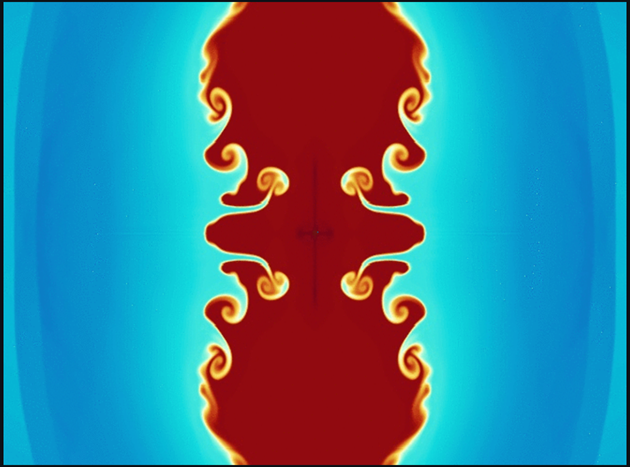
\includegraphics{FVM.png}
    \caption{FVM-Euler方程计算结果}
    \label{fig:FVM}
    \end{figure}


\begin{figure}[t]
    \centering
    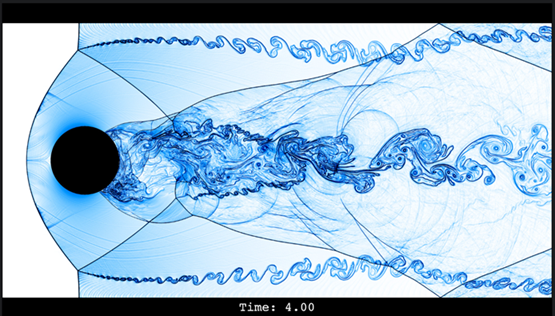
\includegraphics{DG.png}
    \caption{DG-Euler方程计算结果}
    \label{fig:DG}
    \end{figure}

Kokkos具体的技术其实主要是利用这个架构,真正意义上的预处理,GMG,AMG,之类的东西是没有的,
基本上就是一个SOR,BlockJacobi作为预处理,简单看了一下,规整网格,写了一个读取配置的,
输出vti的,好处是可以开启SIMD加速,以及可以在GPU上跑,但其实我觉得没有好的预处理感觉
规模稍微大点就是一眼寄。 

DG比较抽象,涉及到分块矩阵的预处理,正交补,以及这个方程本身就是个非线性方程,一般牛顿-
辛普森方程的雅可比矩阵还得处理一下,时变问题的CN离散方法,顺便一提这位直接不想写非线性
的雅可比,使用是自动微分,主打一个看不懂,以及网格自适应(只能说还好不是p自适应)

顺便一说,这东西我是纯粹看个乐子,主打一手开心,顺便比较一下FVM和DG的差别,目前按照我的理解
,FVM是0阶的DG,但我印象里面DG对于第一类边界条件是添加在弱形式里面,或者加上惩罚,不知道
FVM的边界是什么情况。为了能够看明白这个东西,将会从比较简单的运输方程到斯托克斯到ins,最后到
Euler,至于什么迎风修正,SUPG之类后面再看看。

将从DG开始,看看这个运输方程是怎么解的,到时候会对比一下连续单元和DG单元的计算结果,看看表面
的跳动怎么样。至于说流体力学是什么,我反正不知道,我只会方程离散到弱形式,为什么这样,以及一些结论可谓
一窍不通,单纯的从方程到离散求解的过程。关于自动微分之前解非线性的时候用过一两回,我只能说用过的
都说好,求什么变分导数,感觉不如残差线性化,尤其对于两相流这样的几个方程套在一起,再掺和一个
水平集描述,可谓是群贤毕至,满汉全席,为了身心健康着想,还是自动微分实在,放弃智力,拥抱现代
c++模板。

最后看看能不能衔接上occt参数化建模优化一下经典的翅膀形状,又是最不想动脑的一集,直接自动微分,
时变问题直接离散伴随,优化LP,顺便看看能不能调一下Tpetra让代码在GPU上跑跑。

\subsubsection{Kokkos - Linear advection equation}
将从对流方程开始坐牢,这个方程的形式不算复杂,主要是使用连续FEM和离散FEM进行计算验证,
众所周知,对于这个双曲方程来说,连续的FEM计算结果会出现非常的的震荡,并且这种震荡不会
随着网格的细化而改善,主要原因是对流方程只约束了速度场的某一个方向导数上的值,但对于
对应的正交方向没有约束,导致如果在边界或这某处出现震荡,这个震荡会沿着特征线扩散到
起点处。

首先来看一下SUPG修正后的连续FEM计算方法,所有内容都只是图个乐,看个乐子。首先是方程形式:
\[
    \beta(x,y,z) \nabla u = f \qquad u = g \ , \quad u\in \partial \Omega_{-}
\]
在上述的方程中,$\beta(x,y,z)$是一个向量场,会随着位置的变化而变化,边界$\partial\Omega_{-}$
是入口边界,满足条件是$\{p\in\partial\Omega : \beta(p) \cdot \mathbf{n} < 0\}$,其实就是入口
边界,然后开始离散化,SUPG格式是迎风流线稳定,具体做法就是试探函数取为$v+\delta\beta\nabla v$,
,对于边界上的测试函数是完全看不明白,基本上就是推导半天得到的结论,取$\beta \cdot\mathbf{n} v$
作为边界测试函数,书上这么说,我也这么写,最不想看懂的一集。

所以上述说完基本上整个离散就结束了,最不想看懂的一集,别管怎么来的,先拿来用用看好不好,两边同时
乘以测试函数并进行积分,如下:
\[
\begin{aligned}
    \int_{\Omega} (v+\delta \beta \nabla v)\cdot \beta \nabla u - 
    \int_{\partial\Omega_{-}} \beta\cdot \mathbf{n} v u =
    \int_{\Omega} (v+\delta \beta \nabla v) f -
    \int_{\partial\Omega_{-}} \beta\cdot \mathbf{n} v g
\end{aligned}
\]
离散完成后就基本上按照上述进行计算即可,其实如果去掉边界的相,单纯的看原始方程的SUPG离散格式,
可以倒退到原始的强形式为$\beta \nabla v + \delta \nabla \cdot [\beta \cdot (\beta\cdot \nabla u)]=0$
,基本上就是多加了个扩散项,但又不是太大的扩散项,具体大小和网格的尺寸相关,也就是$\delta(h)$

对于DG方法来说,还是需要需要稳定项,但只是在内部边界上,
离散起来更为简洁,但是DG对于第一类边界条件要么加到弱形式里面,要么
加入惩罚,处理起来比较抽象。离散格式如下:
\[
    \begin{aligned}
        \int_{\Omega} v \beta \nabla u &= \int_{\partial\Omega} v \beta \cdot \mathbf{n} u -
        \int_{\Omega} u \beta \nabla v \\
        &= \int_{\partial\Omega_{-}} v \beta \cdot \mathbf{n} g + 
           \int_{\partial\Omega_{+}} v \beta \cdot \mathbf{n} u +
           \int_{\partial\Omega_{inner}} [v] \beta \cdot \mathbf{n} u^{upwind} -
           \int_{\Omega} u \beta \nabla v
    \end{aligned}
\]

\section{Trilinos 学习}
\subsection{Trilinos Panzer}

Trilinos是和Petsc类似的HPC计算基本库,相比Petsc来说,Trilinos项目更大,代码更加现代化,
特指c++模板一堆,这个有好有坏,学习成本比较高,但是功能非常强大,用户层面比较高,可以
专注于功能的实现,不需要考虑不同架构上的性能问题(最新一代的矩阵向量Tpetra建立在Kokkos上)
。Petsc使用c语言实现,核心功能非常明确矩阵Mat,向量Vec,线性求解器Ksp,非线性求解器Sens,
时间积分求解Ts,优化求解Tao,个人建议最好配置的时候外部配置一下SUNDIALS,提供一系列时间积分
求解方法以及切线敏度和伴随敏度分析。

以下是从官网上扣下来的几个模块的介绍,计算效率比手写的高出一大截()
\begin{itemize}
  \item ARKODE, a solver with one-step methods for stiff, nonstiff, mixed stiff-nonstiff, and multirate ODE systems.
  \item CVODE, a solver with Adams and BDF methods for stiff and nonstiff ODE systems.
  \item CVODES, an extension of CVODE with forward and adjoint sensitivity analysis capabilities for stiff and nonstiff ODE systems.
  \item IDA, a solver with BDF methods for DAE systems.
  \item IDAS, an extension of IDA with forward and adjoint sensitivity analysis capabilities for DAE systems.
  \item KINSOL, a solver for nonlinear algebraic systems.
\end{itemize}
Petsc中Ts也提供许多时间积分求解器,如BDF,$\theta$法,RK,IMEX等,最近提供了伴随导数的计算,
以及伪时间步进方法。

说了这么多Petsc相关的内容,Trilinos里面有什么不同吗?,确实不同,上面所说的内容,Trilinos里面都提供,
甚至还有更多。Petsc本身并不提供特征值计算,Slepc作为Petsc的外延,提供基于子空间投影方法的特征值计算
方案。以我的使用体验,低网格数下,Petsc效率比Trilinos略高一点,但高网格和复杂方程下,Petsc的编写成本
会非常高,计算效率比Trilinos低不少。这里不是因为Petsc本身的计算效率不高,而是因为对于复杂PDE来说,
计算Jacobian和求解线性系统非常耗时,手写代码效率一般。

其次还有一点,Trilinos提供自动微分,在实现计算的同时,通过模板改变数值类型可以做到自动求解Jacobian,
只需要将弱形式编写完成,对应的Jacobian可以使用自动微分计算。最后,Petsc的不提供有限元,有限体,有限差分
等方法的实现,需要自己手动编写。上限自然是有的,但取决于个人的代码水平。如果你对openmpi,openmp,simd非常
理解,能够避免并行计算的常见错误,提高计算效率,自然计算效率很高。但其实大伙都不怎么会,写出来的基本上也就是
能跑的水平,至于性能不是重点,更关注方程和收敛性。这时Trilinos的优势就凸显出来。

\subsubsection{Trilinos Tpetra MultiVector and CrsMatrix}
这段时间一直没更新主要是在看SUPG和DG,以及重新编译安装Trilinos,之前安装的版本缺少
一些内容,没有网格输入输出(STK)和自由度管理(Panzer)。给我折磨坏了,最新release版本有问题,方程
离散工具和自由度管理工具之间出现重复定义导致编译不通过,还得克隆下来master然后重新
安装,目前应该是完全的安装好了。

可能会比较迷惑的点在与Kokkos和Trilinos为啥会混合在一起,实际上Kokkos是Trilinos的
一个子项目,也是最核心的底层架构,主要负责矩阵向量表示,稀疏矩阵计算。Tpetra就是
以Kokkos为核心的线性代数核心包,因为网上的Trilinos介绍非常少,在此处简单的列举
安装上的核心库的主要作用。

\begin{itemize}
    \item Kokkos/KokkosKernels 核心底层
    \item Tpetra/Xpetra        线性代数表示/抽象接口
    \item Teuchos              提供参数文件/命令行参数,智能指针,MPI接口
    \item Amesos2              提供外部的稀疏直接求解器,MUMPS,SuperLU,UMPACK
    \item Anasazi              特征值计算
    \item Belos                提供各种迭代方法,包括无矩阵接口
    \item Galeri               提供有限差分法离散
    \item ifpack2              提供一般的预处理,SOR,Jacobian之类
    \item Intrepid2            提供旋度场,散度场,梯度场离散,基函数,正交规则
    \item ...  
\end{itemize}

这里面有必要着重提及Sacado和Muelu,后者是提供平滑聚类多重网格个几何多重网格的包,
前者是用于实现自动微分功能(尤其对于材料非线性,
多相流,敏度分析这些东西),你开始计算一个非线性材料的传热性能,辛辛苦苦推导出了对应
的Jacobian方程,输入到对应的牛顿方法中,进行计算。你觉得这套方案一定能够适用其他问题,
直到你遇到了多相流,参数敏度,你开始熬夜手搓,突然发现可以直接放弃大脑,拥抱现代c++。

Sacado提供正向直接微分和反向伴随微分,微分精度为机器精度,同时和Tpetra矩阵向量通过
模板结合,可以直接在cuda上跑。什么你说不是手动推导的没有灵魂,确实没有灵魂,但你手动
推导直接切线方程和伴随方程还没结束,这边可能就编写求解代码,边重载计算敏度了,折磨自己
不如折磨机器()

如果你安装了Sacado,以下是一个小测试案例

\begin{lstlisting}
#include <Sacado.hpp>
#include <iostream>
using fad_double = Sacado::Fad::DFad<double>;
int main() {
  fad_double a,b,c;
  a = 1; b = 2;
  a.diff(0,2);  // Set a to be dof 0, in a 2-dof system.
  b.diff(1,2);  // Set b to be dof 1, in a 2-dof system.
  c = 2*a+cos(a*b);
  double *derivs = &c.fastAccessDx(0); // Access derivatives
  double a_value = 1, b_value = 2;
  double dc_da = 2 - sin(a_value * b_value) * b_value;
  double dc_db = - sin(a_value * b_value) * a_value;
  std::cout << std::setprecision(16) << "Sacado : dc/da = " << derivs[0] << ", dc/db=" << derivs[1] << std::endl;
  std::cout << std::setprecision(16)<< "Hands  : dc/da = " << dc_da << ", dc/db=" << dc_db << std::endl;
}
\end{lstlisting}

其对应的输出结果如下:
\[
\begin{aligned}
Sacado &: dc/da = 0.1814051463486366, dc/db=-0.9092974268256817\\
Hands  &: dc/da = 0.1814051463486366, dc/db=-0.9092974268256817    
\end{aligned}
\]

对于大型的离散问题来说,使用自动微分对整个矩阵进行计算似乎是不是非常的现实,
但实际情况是,不会直接对整个稀疏矩阵进行计算,而是对每个单元刚度矩阵进行微分
再进行组合,使用c++模板重载实现在计算总体矩阵的时候同时计算Jacobian矩阵。对于
参数敏度更是如此,放弃智力,拥抱现代c++

以下代码是使用Galeri进行Laplace方程的有限差分离散,主要是需要搞明白矩阵向量的初始化。

\begin{lstlisting}
#include "Galeri_XpetraMaps.hpp"
#include "Galeri_MatrixTraits.hpp"
#include "Galeri_XpetraMatrixTypes.hpp"
#include "Galeri_XpetraProblemFactory.hpp"
#include "Teuchos_DefaultComm.hpp"
#include "Teuchos_ParameterList.hpp"

#define GO long long
#define Scalar int
#define LO int
#define Node Tpetra::KokkosCompat::KokkosOpenMPWrapperNode

using namespace Galeri;
int main(int argc, char *argv[])
{
    using Teuchos::RCP;
    using Teuchos::rcp;
    typedef Tpetra::Map<LO, GO, Node> Tpetra_Map;
    typedef Tpetra::CrsMatrix<Scalar, LO, GO, Node> Tpetra_CrsMatrix;
    typedef Tpetra::MultiVector<Scalar, LO, GO, Node> Tpetra_MultiVector;
    typedef Teuchos::ScalarTraits<Scalar> ScalarTraits;
#ifdef HAVE_MPI
    MPI_Init(&argc, &argv);
#endif
    // Create comm
    RCP<const Teuchos::Comm<int>> comm = Teuchos::DefaultComm<int>::getComm();
    // Here we create the linear problem
    //
    //   Matrix * LHS = RHS
    //
    // with Matrix arising from a 5-point formula discretization.
    std::string mapType = "Cartesian2D";
    auto mapParameters = Teuchos::ParameterList("Tpetra::Map");
    // dimension of the problem is nx x ny
    mapParameters.set("nx", 10 * comm->getSize());
    mapParameters.set("ny", 10);
    // total number of processors is mx x my
    mapParameters.set("mx", comm->getSize());
    mapParameters.set("my", 1);
    mapParameters.print();
    auto out = Teuchos::getFancyOStream(Teuchos::rcpFromRef(std::cout));
    try
    {
        // Creation of the map
        auto map = RCP{Galeri::Xpetra::CreateMap<Scalar, GO, Tpetra_Map>(mapType, comm, mapParameters)};
        // Creation of linear problem
        auto problem = Galeri::Xpetra::BuildProblem<Scalar, LO, GO, Tpetra_Map, Tpetra_CrsMatrix, Tpetra_MultiVector>("Laplace2D", map, mapParameters);
        // Build Matrix and MultiVectors
        auto matrix = problem->BuildMatrix();
        auto LHS = rcp(new Tpetra_MultiVector(matrix->getDomainMap(), 1));
        auto RHS = rcp(new Tpetra_MultiVector(matrix->getRangeMap(), 1));
        auto ExactSolution = rcp(new Tpetra_MultiVector(matrix->getDomainMap(), 1));
        ExactSolution->randomize(0, 100);
        LHS->putScalar(ScalarTraits::zero());
        matrix->apply(*ExactSolution, *RHS);
        matrix->describe(*out, Teuchos::EVerbosityLevel::VERB_EXTREME);
        LHS->describe(*out, Teuchos::EVerbosityLevel::VERB_EXTREME);
        RHS->describe(*out, Teuchos::EVerbosityLevel::VERB_EXTREME);
        ExactSolution->describe(*out, Teuchos::EVerbosityLevel::VERB_EXTREME);
        // at this point any LinearSolver can be used which understands the Tpetra objects. For example: Amesos2 or Ifpack2
    }
    catch (Galeri::Exception &rhs)
    {
        if (comm->getRank() == 0)
        {
            cerr << "Caught exception: ";
            rhs.Print();
#ifdef HAVE_MPI
            MPI_Finalize();
#endif
            return (EXIT_FAILURE);
        }
    }
#ifdef HAVE_MPI
    MPI_Finalize();
#endif
    return (EXIT_SUCCESS);
}
\end{lstlisting}

\subsubsection{Galeri, Belos \&\& Ifpack2}
感觉现在刚开始用这套代码,就是纯纯的缝合,先去对应的包里面找教程和案例,再
把这些教程的内容复合在一起,得到需要的东西,刚开始先暂时不考虑组装的问题,
使用Geleri有限差分构建需要的矩阵和向量,Belos线性求解器,Ifpack2预处理器。
先简单实验一下.
\begin{lstlisting}
// Ifpack2
#include <Ifpack2_Factory.hpp>
#include <Ifpack2_Preconditioner.hpp>

// Teuchos
#include <Teuchos_Assert.hpp>
#include <Teuchos_CommandLineProcessor.hpp>
#include <Teuchos_ParameterList.hpp>
#include <Teuchos_StandardCatchMacros.hpp>

// Tpetra
#include <Tpetra_Core.hpp>
#include <Tpetra_CrsMatrix.hpp>
#include <Tpetra_Map.hpp>
#include <Tpetra_MatrixIO.hpp>
#include <Tpetra_MultiVector.hpp>
#include <Tpetra_Operator.hpp>

// Belos
#include "BelosConfigDefs.hpp"
#include "BelosLinearProblem.hpp"
#include "BelosTFQMRSolMgr.hpp"
#include "BelosTpetraAdapter.hpp"

// Galeri
#include <Galeri_XpetraMaps.hpp>
#include <Galeri_XpetraMatrixTypes.hpp>
#include <Galeri_XpetraProblemFactory.hpp>

int main(int argc, char *argv[])
{
    // 浮点数类型
    using ST = typename Tpetra::MultiVector<>::scalar_type;
    // 局部自由度索引类型
    using LO = typename Tpetra::MultiVector<>::local_ordinal_type;
    // 全局自由度索引类型
    using GO = typename Tpetra::MultiVector<>::global_ordinal_type;
    // Kokkos 运行空间
    // 如果安装了CUDA,默认就在CUDA上跑
    // using NT = typename Tpetra::MultiVector<>::node_type;
    // 可以手动选择运行空间
    using NT = typename Tpetra::KokkosCompat::KokkosOpenMPWrapperNode;
    // 线性算子,矩阵的抽象封装
    using OP = typename Tpetra::Operator<ST, LO, GO, NT>;
    // 多重向量
    using MV = typename Tpetra::MultiVector<ST, LO, GO, NT>;

    // 矩阵稀疏模板
    using tmap_t = Tpetra::Map<LO, GO, NT>;
    // 稀疏矩阵
    using tcrsmatrix_t = Tpetra::CrsMatrix<ST, LO, GO, NT>;

    // 定义Belos统一的外部向量封装接口
    using MVT = typename Belos::MultiVecTraits<ST, MV>;
    // 定义Belos统一的外部矩阵封装接口
    using OPT = typename Belos::OperatorTraits<ST, MV, OP>;

    // 浮点数类型当前的具体类型
    using MT = typename Teuchos::ScalarTraits<ST>::magnitudeType;
    // 浮点数类型的抽象封装
    using STM = typename Teuchos::ScalarTraits<MT>;

    // 定义线性问题
    using LinearProblem = typename Belos::LinearProblem<ST, MV, OP>;
    // 定义预处理器
    using Preconditioner = typename Ifpack2::Preconditioner<ST, LO, GO, NT>;
    // 线性求解器
    using TFQMRSolMgr = typename Belos::TFQMRSolMgr<ST, MV, OP>;

    // 智能指针
    using Teuchos::RCP;
    using Teuchos::rcp;
    // 参数文件
    using Teuchos::ParameterList;

    Tpetra::ScopeGuard MyScope(&argc, &argv);
    {
        RCP<const Teuchos::Comm<int>> comm = Tpetra::getDefaultComm();
        // RCP<Teuchos::FancyOStream> Myout = Teuchos::getFancyOStream(Teuchos::rcpFromRef(std::cout));

        // Flag 是否使用左预处理
        bool leftPrec = true;
        // Int 参数决定RHS的个数
        int RhsNum = 1;
        // 迭代容差
        MT tol = STM::squareroot(STM::eps());

        // 网格的点数
        int nx = 100;

        // 命令行参数控制
        Teuchos::CommandLineProcessor cmdp(false, true);
        cmdp.setOption("LeftPrec", "RightPrec", &leftPrec, "Preconditioner Type");
        cmdp.setOption("RHSnum", &RhsNum, "Number Of RHS");
        cmdp.setOption("nx", &nx, "Number Of Grid");
        if (cmdp.parse(argc, argv) != Teuchos::CommandLineProcessor::PARSE_SUCCESSFUL)
        {
            return EXIT_FAILURE;
        }

        // 通过Galeri创建稀疏模板,并填充数据
        ParameterList GaleriList;
        GaleriList.set("n", nx * nx * nx);
        GaleriList.set("nx", nx);
        GaleriList.set("ny", nx);
        GaleriList.set("nz", nx);
        GaleriList.set("mx", (int)comm->getSize());
        GaleriList.set("my", 1);
        GaleriList.set("mz", 1);
        // 稀疏模板
        RCP<tmap_t> MatrixMap =
            RCP{Galeri::Xpetra::CreateMap<LO, GO, tmap_t>("Cartesian3D", comm, GaleriList)};
        // 稀疏矩阵类型
        auto GaleriProblem =
            Galeri::Xpetra::BuildProblem<ST, LO, GO, tmap_t, tcrsmatrix_t, MV>("Laplace3D", MatrixMap, GaleriList);
        // 创建稀疏矩阵并计算
        RCP<tcrsmatrix_t> MyMatrix = GaleriProblem->BuildMatrix();

        // 创建右端项
        RCP<MV> MyRHS = rcp(new MV(MatrixMap, RhsNum));
        // 创建解向量
        RCP<MV> MySolution = rcp(new MV(MatrixMap, RhsNum));
        // 创建正确的解向量
        RCP<MV> MyExSolution = rcp(new MV(MatrixMap, RhsNum));
        // 将解向量随机化
        MVT::MvRandom(*MyExSolution);
        // RHS = A * EXSolution
        OPT::Apply(*MyMatrix, *MyExSolution, *MyRHS);

        // 设定Ifpack2 ILU预处理器
        std::string precType = "RILUK";
        RCP<Preconditioner> prec = Ifpack2::Factory::create<tcrsmatrix_t>(precType, MyMatrix);
        
        TEUCHOS_ASSERT(prec != Teuchos::null);

        // 预处理参数
        int lFill = 2;
        int overlap = 2;
        ST absThresh = 0.0;
        ST relThresh = 1.0;

        ParameterList precParams;
        precParams.set("fact: iluk level-of-fill", lFill);
        precParams.set("fact: iluk level-of-overlap", overlap);
        precParams.set("fact: absolute threshold", absThresh);
        precParams.set("fact: relative threshold", relThresh);
        prec->setParameters(precParams);
        // 初始化预处理器并计算具体值
        prec->initialize();
        prec->compute();

        int MaxIters = MyRHS->getGlobalLength() - 1;
        // 设定线性求解器
        ParameterList belosList;        
        belosList.set("Maximum Iterations", MaxIters);
        belosList.set("Convergence Tolerance", tol);    
        belosList.set("Explicit Residual Test", true); 
        belosList.set("Verbosity", 
                       Belos::Errors + 
                       Belos::Warnings + 
                       Belos::TimingDetails + 
                       Belos::StatusTestDetails);

        // 定义线性问题
        RCP<LinearProblem> MyProblem = rcp(new LinearProblem(MyMatrix,MySolution,MyRHS));
        if (leftPrec)
        {
            MyProblem->setLeftPrec(prec);            
        }
        else
        {
            MyProblem->setRightPrec(prec);  
        }

        bool set = MyProblem->setProblem();
        if (set == false)
        {
            std::cout << std::endl
                          << "ERROR:  Belos::LinearProblem failed to set up correctly!" << std::endl;
            return EXIT_FAILURE;
        }
        
        // 创建线性求解器
        RCP<TFQMRSolMgr> MySolver = rcp(new TFQMRSolMgr(MyProblem,rcp(&belosList,false)));
        
        std::cout << "Solving..." << std::endl;
        Belos::ReturnType ret = MySolver->solve();
        std::cout << "Solve end" << std::endl;

        // 将求解的解和真解对比
        bool badRes = false;
        std::vector<ST> actualResids(RhsNum);
        std::vector<ST> rhsNorm(RhsNum);

        // 残差向量
        MV resids(MatrixMap, RhsNum);
        // r = A*x - b
        OPT::Apply(*MyMatrix, *MySolution, resids);
        MVT::MvAddMv(-1.0, resids, 1.0, *MyRHS, resids);
        // 
        MVT::MvNorm(resids, actualResids,Belos::TwoNorm);
        MVT::MvNorm(*MyRHS, rhsNorm);
        // 
        std::cout << "---------- Actual Residuals (normalized) ----------" << std::endl
                    << std::endl;
        for (int i = 0; i < RhsNum; i++)
        {
            ST actRes = actualResids[i] / rhsNorm[i];
            std::cout << "Problem " << i << " : \t" << actRes << std::endl;
            if (actRes > tol)
                badRes = true;
        }
        // 
        if (ret != Belos::Converged || badRes)
        {
            std::cout << std::endl
                          << "ERROR:  Belos did not converge!" << std::endl;
        }
        else
        {
            std::cout << std::endl
                          << "SUCCESS:  Belos converged!" << std::endl;
        }
    }
    return EXIT_SUCCESS;
}
\end{lstlisting}

\newpage
\begin{table}[htbp]
\setlength{\tabcolsep}{8mm}
\begin{tabular}{ccccc}
\hline
\multicolumn{1}{|c|}{\textbf{MPI/CUDA Run time}} & \multicolumn{1}{c|}{\textbf{Serial}} & \multicolumn{1}{c|}{\textbf{MPI NP 2}} & \multicolumn{1}{c|}{\textbf{MPI NP 4}} \\ \hline
\multicolumn{1}{|c|}{\textbf{CUDA}} & \multicolumn{1}{c|}{4.78s} & \multicolumn{1}{c|}{1.89s} & \multicolumn{1}{c|}{1.43s} \\ \hline
\multicolumn{1}{|c|}{\textbf{OpenMP}} & \multicolumn{1}{c|}{2.5s} & \multicolumn{1}{c|}{1.94s} & \multicolumn{1}{c|}{1.72s} \\ \hline
\end{tabular}
\caption{MPI/Serial CUDA/OpenMP 运行时间}
\end{table}
默认情况下$nx=100$且是三维问题,网格数量就是$nx^3$,自由度数量也是差不多的量级。
预处理器使用$ILU$预处理。以下是具体的细节时间输出

\begin{table}[htbp]
\setlength{\tabcolsep}{5mm}
\begin{tabular}{lllll}
\hline
\multicolumn{1}{|c|}{\textbf{Timer Name}} & \multicolumn{1}{c|}{\textbf{MinOverProcs}} & \multicolumn{1}{c|}{\textbf{MeanOverProcs}} & \multicolumn{1}{c|}{\textbf{MaxOverProcs}}  \\ \hline
\multicolumn{1}{|c|}{\textbf{Op*x}} &         \multicolumn{1}{|c|}{0.1789}        &                  \multicolumn{1}{|c|}{ 0.2399}             &                 \multicolumn{1}{|c|}{0.2789}                      \\ \hline
\multicolumn{1}{|c|}{\textbf{Prec*x}} &        \multicolumn{1}{|c|}{ 0.9508}        &               \multicolumn{1}{|c|}{0.9579}                 &               \multicolumn{1}{|c|}{0.9669}                                            \\ \hline
\multicolumn{1}{|c|}{\textbf{TFQMRSolMgr}} &   \multicolumn{1}{|c|}{1.432}        &           \multicolumn{1}{|c|} {1.435}                    &             \multicolumn{1}{|c|}{1.438}             \\ \hline
\multicolumn{1}{|c|}{\textbf{fillComplet}} &   \multicolumn{1}{|c|}{0.133 }       &            \multicolumn{1}{|c|}{0.1361}          &              \multicolumn{1}{|c|}{0.1372}                  \\ \hline
\multicolumn{1}{|c|}{\textbf{generation}} &     \multicolumn{1}{|c|}{0.08773}        &           \multicolumn{1}{|c|}{0.089}            &               \multicolumn{1}{|c|}{0.09294}                     \\   \hline                   
\end{tabular}
\caption{具体运行时间}
\end{table}

时间消耗最长的是预处理器的计算和预处理器和向量的计算,在CUDA上计算的优势就是可以大幅的
加速矩阵向量乘法的计算效率,可以得到非常明显的加速效果,CPU上由于不同节点之间的相互通信
以及带宽的限制,加速效果具有明显的边际效应。在800w网格下的计算时间为
\[
\begin{aligned}
    mpirun\ -np\ 4\ \&\&\ CUDA &:\ 33.26s\\
    mpirun\ -np\ 4\ \&\&\ OpenMP &:\ 25.56s\\
\end{aligned}
\]
此处OpenMP的计算速度快于CUDA的原因非常简单,(CUDA内存太小了,任务管理器显示内存使用满了)

\subsubsection{Panzer Laplace Example}
Panzer 是Trilinos的复合物理场的统一管理包,可以耦合多个物理场,但这个使用起来比较抽象,
这个模块设计的时候是考虑到了线性和非线性的问题,将一系列物理场进行耦合。如果还记得之前
的自动微分包Sacado,在进行刚度矩阵计算的时候,会通过重载基类进行计算,计算的数值类型包括了
三种$double,Sacado::Fad::DFad<double>$,正常计算有限元问题的时候就使用$double$,如果
需要对问题进行非线性求解,就将计算类型的模板给定为$Sacado::Fad::DFad<double>$,两者
使用的是同一套模板函数,这个设计也就是之前提到的计算单元刚度矩阵的同时计算$Jacobian$

Panzer包括$DOFManager,ConnManager,ClosureModelManager,FieldManager$,这四个的作用包括网格管理,自由度管理,物理场管理和求解模型管理。因为代码有点多,没法一次性
放到PDF上,所以只挑选其中一部分代码进行解释网格和自由度先不看,以Laplace方程为例理解物理场
是如何进行计算和离散的。以下说明以Laplace方程和时变Laplace方程举例。

\begin{lstlisting}
struct Residual { typedef RealType ScalarT; };
\end{lstlisting}
\[
\begin{aligned}
    \nabla\cdot (c(u) \cdot u) = Q \\
    R = \nabla u \cdot c(u) \cdot\nabla v - Q \\
\end{aligned}
\]
上述问题为一个非线性的Laplace问题,其中$c(u)$表示和自变量$u$相关的分部场,$R$为离散化的求解方程。

\begin{lstlisting}
struct Jacobian { typedef FadType  ScalarT; };
\end{lstlisting}
\[
\begin{aligned}
    J &= \frac{\partial R}{\partial u} \\
      &= \lim_{\epsilon\rightarrow 0}\frac{1}{\epsilon}
        (R(u+\epsilon \delta u) - R(u))\\
      &= \lim_{\epsilon\rightarrow 0}\frac{1}{\epsilon}
         (\nabla (u+\epsilon \delta u) \cdot c(u+\epsilon \delta u)\cdot \nabla v 
        -\nabla u \cdot c(u) \cdot\nabla v) \\
      &= \nabla \delta u \cdot c(u) \cdot\nabla v + 
          \nabla u\cdot c(u)_u \cdot \delta u \cdot \nabla v
\end{aligned}
\]
对于这个非线性问题来说,进行空间离散后会形成如$A(u)u=Q$的形式,为了求解这个非线性问题,一般使用
牛顿方法进行计算$R(u)+J \delta u = 0$,这样迭代到收敛,类似的
方法还有许多的变种,但一般这个就够用了。

\begin{lstlisting}
struct Tangent  { typedef FadType  ScalarT; };
\end{lstlisting}
Tangent 敏度分析,以时变问题为例,p为参数
\[
\begin{aligned}
\frac{\partial u}{\partial t} &= \nabla u\cdot c(p)\cdot \nabla v + Q\\
\frac{u^n-u^{n-1}}{\Delta t} &= \nabla u^{n-1}\cdot c(p)\cdot \nabla v + Q\\
(\frac{\partial u^n}{\partial p} - \frac{\partial u^{n-1}}{\partial p})&= 
\Delta t\nabla u^{n-1} \cdot\frac{\partial c}{\partial p} \cdot\nabla v +
\Delta t \nabla v \cdot c \cdot \nabla v \frac{\partial u^{n-1}}{\partial p}
\end{aligned}
\]
以简单的差分格式举例,通过给定0时刻下的敏度初值,带入上述方程进行迭代可以计算得到最终时刻下的敏度,
敏度扩散顺序和
时间迭代顺序一致,一般被称为Tangent。和这个方程相对应的是伴随模型Adjoint,其敏度扩散顺序和
时间迭代顺序相反,这两中方案只是求导的
顺序不同,但是求解的结果是完全一致的,Tangent适用于参数个数比较少,优化目标比较多的情况,
Adjoint适用于参数个数比较多,优化目标比较少的情况。

EvalT 为实际计算的类型,主要包括两种选择正常计算使用的浮点数类型double,float非线性问题使用的自动微分类型FadType
这个类的初始化方法需要传入参数文件,积分阶次,网格数据和全局的自由度数据,$build\_transient\_support$表示
是否计算瞬态问题
\begin{lstlisting}
template <typename EvalT>
Example::PoissonEquationSet<EvalT>::
    PoissonEquationSet(const Teuchos::RCP<Teuchos::ParameterList> &params,
                       const int &default_integration_order,
                       const panzer::CellData &cell_data,
                       const Teuchos::RCP<panzer::GlobalData> &global_data,
                       const bool build_transient_support)
: panzer::EquationSet_DefaultImpl<EvalT>(params, 
                                         default_integration_order, 
                                         cell_data, 
                                         global_data, 
                                         build_transient_support)
{
...
}
\end{lstlisting}

这个部分设计的比较抽象,首先回忆一下正常的Laplace方程弱形式离散,正如上面写的,单元
刚度矩阵为$\nabla v\cdot c \cdot\nabla v$的双线性形式,故此选定的基函数为$HGrad$,在
添加完温度场后,再添加对应的梯度场.
\begin{lstlisting}
// 创建一个新的参数列表,给出默认的参数值,和传入的参数列表进行匹配
// 如果传入没有这个参数则会加入进去
Teuchos::ParameterList valid_parameters;
this->setDefaultValidParameters(valid_parameters);

valid_parameters.set("Model ID", "", "Closure model id associated with this equaiton set");
valid_parameters.set("Basis Type", "HGrad", "Type of Basis to use");
valid_parameters.set("Basis Order", 1, "Order of the basis");
valid_parameters.set("Integration Order", -1, "Order of the integration rule");

params->validateParametersAndSetDefaults(valid_parameters);
// 获取参数
std::string basis_type = params->get<std::string>("Basis Type");
int basis_order = params->get<int>("Basis Order");
int integration_order = params->get<int>("Integration Order");
std::string model_id = params->get<std::string>("Model ID");

// 这里声明创建一个TEMPERATURE的物理场
this->addDOF("TEMPERATURE", basis_type, basis_order, integration_order);
// 因为基函数类型为HGrad,这里需要温度场的梯度
this->addDOFGrad("TEMPERATURE");
// 如果计算瞬态问题,需要DTEMPERATURE_DT
if (this->buildTransientSupport())
  this->addDOFTimeDerivative("TEMPERATURE");
// 将边界条件,物理区域组合起来
this->addClosureModel(model_id);

this->setupDOFs();
\end{lstlisting}

我们再来看添加完成自由度之后,如何实现离散化.Panzer的封装程度非常高,
正常理解的组装过程可能是循环所有的网格,在每个网格上根据基函数确定梯度值,
根据积分规则和阶数确定正交点,循环所有正交点,计算双线性形式,再根据实际网格
尺寸计算等参变换的$Jacobian$矩阵和对应的行列式,最后根据全局自由度索引提交
到总刚度矩阵上.

这个过程是一般的有限元计算流程,但如何让这个过程更快?可以看到在参考单元上计算
$\nabla\cdot v$的时候,所有单元(如果不考虑混合网格)是完全一致的,可以把这部分
分离出来,所有网格只需要计算一次.Panzer的离散过程就只需要指定基函数乘以
那一部分即可,其余过程可以自动进行.
\begin{lstlisting}
// 积分阶次
RCP<IntegrationRule> ir = this->getIntRuleForDOF("TEMPERATURE");
// 基函数类型
RCP<BasisIRLayout> basis = this->getBasisIRLayoutForDOF("TEMPERATURE");
// 定义瞬态项算子
if (this->buildTransientSupport())
{
  // 残差R的名称,需要计算的v \dot Scalar中的Scalar对应的项
  string resName("RESIDUAL_TEMPERATURE"), 
         valName("DXDT_TEMPERATURE");
  double multiplier(1);
  // 此处不需要给出v的具体形式,只要给出
  // v \dot Scalar中的Scalar对应的项即可
  // 相当于v \dot DXDT_TEMPERATURE 
  RCP<Evaluator<Traits>> op = 
      rcp(new Integrator_BasisTimesScalar<EvalT, Traits>
                  (EvaluatorStyle::CONTRIBUTES,
                   resName, valName, *basis, *ir, multiplier));
  // 创建这个算子
  this->template registerEvaluator<EvalT>(fm, op);
}

// 定义扩散项算子 \int \nabla T \cdot \nabla v
{
  double thermal_conductivity = 1.0;

  ParameterList p("Diffusion Residual");
  p.set("Residual Name", "RESIDUAL_TEMPERATURE");
  p.set("Flux Name", "GRAD_TEMPERATURE");
  p.set("Basis", basis);
  p.set("IR", ir);
  p.set("Multiplier", thermal_conductivity);
  // \nabla v \cdot Vec,Vec给定为GRAD_TEMPERATURE
  RCP<Evaluator<Traits>> op = 
        rcp(new Integrator_GradBasisDotVector<EvalT, Traits>(p));

  this->template registerEvaluator<EvalT>(fm, op);
}

// 源项
{
  string resName("RESIDUAL_TEMPERATURE"),
         valName("SOURCE_TEMPERATURE");
  double multiplier(-1);
  // v \cdot Scalar, Scalar给定为Q
  RCP<Evaluator<Traits>> op = 
      rcp(new Integrator_BasisTimesScalar<EvalT, Traits>
                  (EvaluatorStyle::CONTRIBUTES,
                  resName, valName, *basis, *ir, multiplier));
  this->template registerEvaluator<EvalT>(fm, op);
}
\end{lstlisting}

\subsubsection{Convection Equation Example}



\end{document}